\section{Design And Implementation}
\label{sec:design}

\todo[inline]{Discuss how the software works.  Things like using CCI for small messages, bulk transfers happening by way of cudaMemcpy().  Mention Cray-specific stuff such as setting 'feature=gpudefault' in the qsub script. }

\todo[inline]{Somewhere in here, we're going to want to insert the graph of host-to-gpu bandwidth vs. transfer size.  It justifies chosing 16MB bocks and we're going to want to reference it from the analysis section, too.}

\subsection{Overview}
\label{subsec:overview}
This idea was tested using a synthetic benchmark application written by the authors.  The benchmark consists of two executables: the main executable which uses MPI and simulates the I/O patterns of a typical HPC application and a daemon process that is started on each compute node.  The daemon has two tasks: manage the GPU memory and copy data from GPU memory out to a file.  Note that the daemon does \emph{not} copy the data into the GPU memory.  There needs to be exactly one daemon process on each compute node regardless of how many MPI ranks are running on each node.  \footnote{Due to the limitations of aprun, starting this daemon is somewhat involved.  See section \ref{subsec:cray-specific}.}

With the daemon process running on each node, the application begins its main execution.  In this case, since it's just a synthetic 
I/O benchmark, it performs no actual computation; it simply writes a specified amount of data and then sleeps for a specified amount of time.  For these tests, the sleep time was deliberately calculated to allow enough time for the data in GPU memory to drain.



\begin{figure*}[!t]
\centerline{
  \subfloat[Application sends write request message to daemon]{
    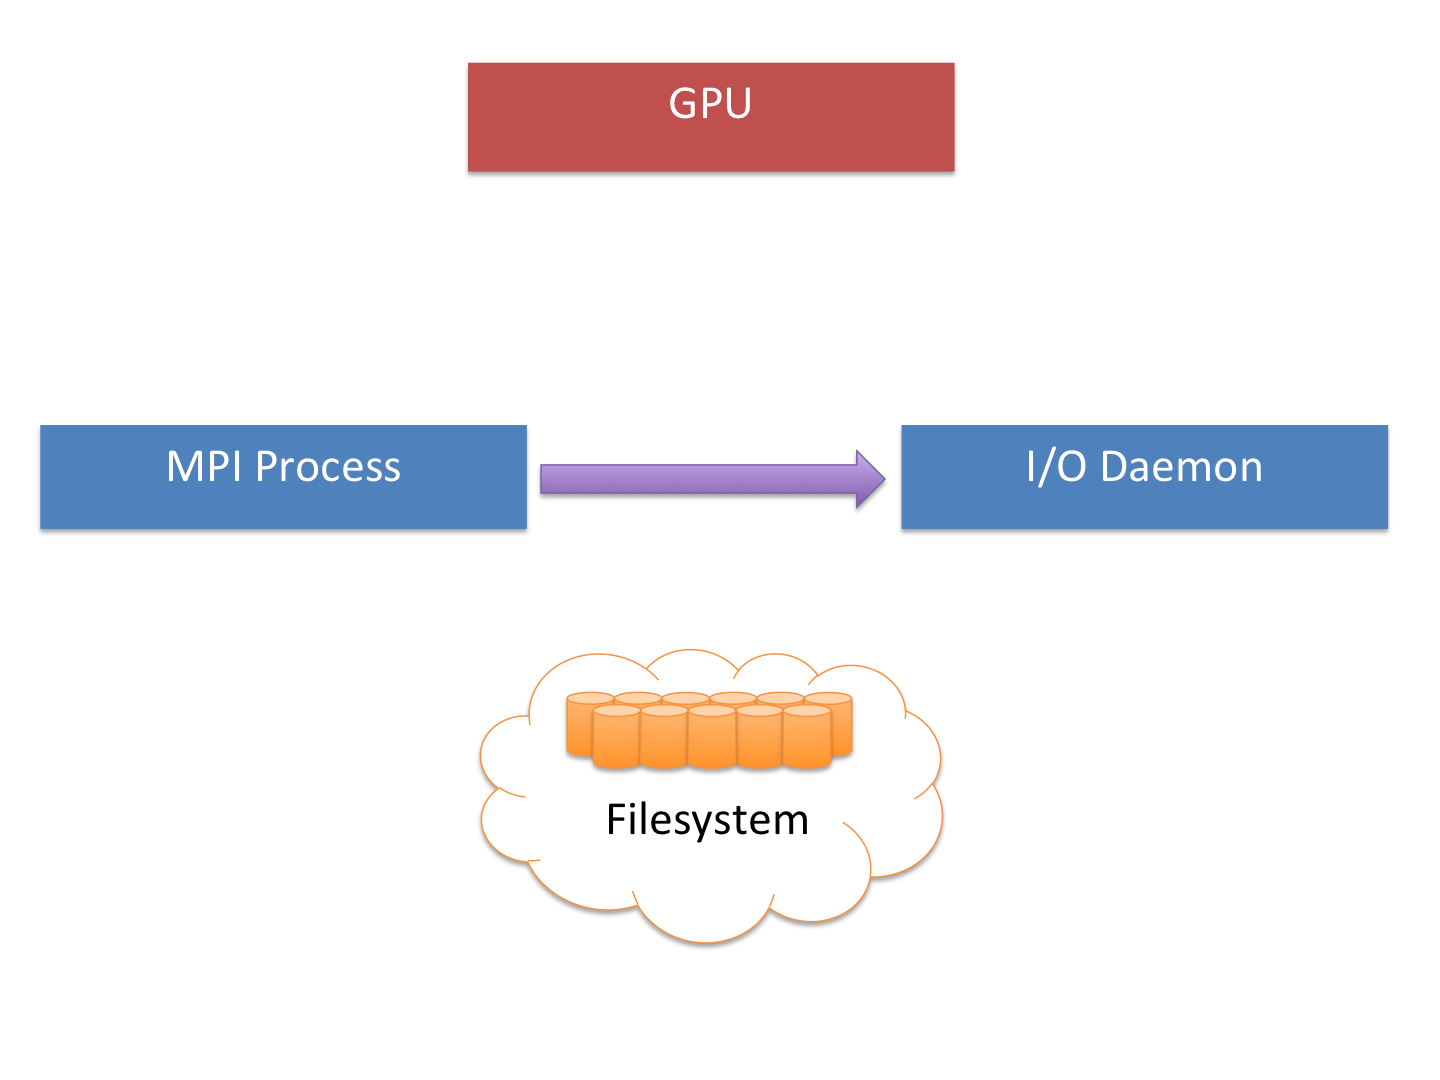
\includegraphics[width=2.5in]{figures/Data_Movement/Slide09}%
    \label{fig:comm_a}}
  \hfil
  \subfloat[Daemon allocates GPU memory and converts pointer into IPC handle]{
    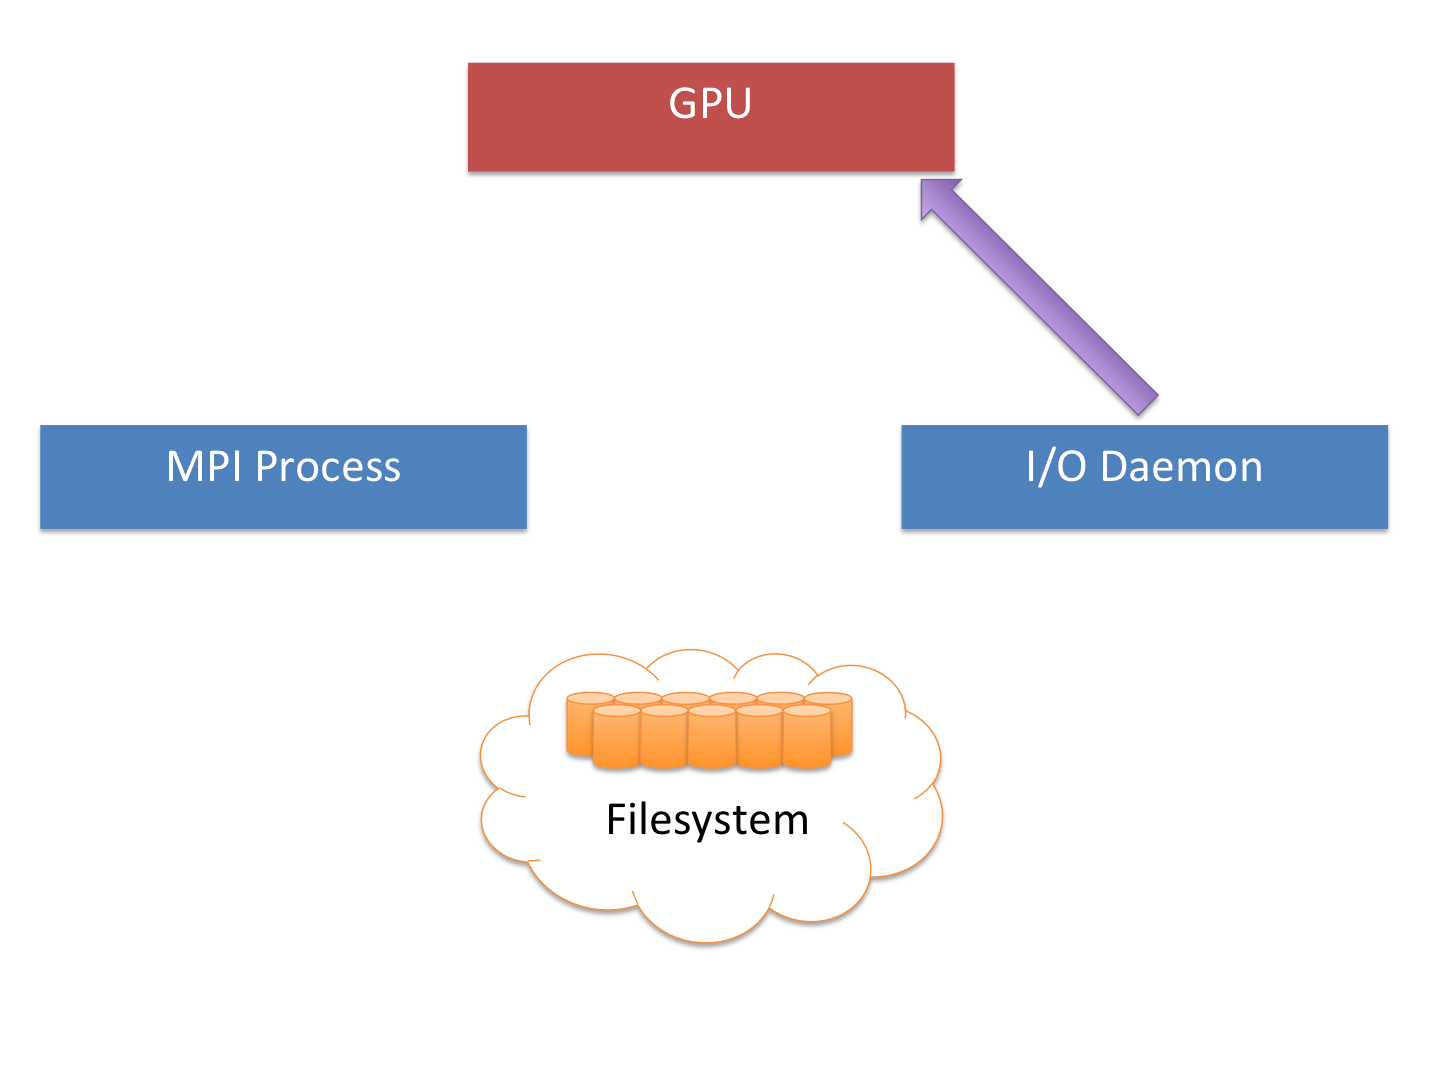
\includegraphics[width=2.5in]{figures/Data_Movement/Slide10}%
    \label{fig:comm_b}}}
\centerline{
  \subfloat[Daemon sends reply message with IPC handle]{
    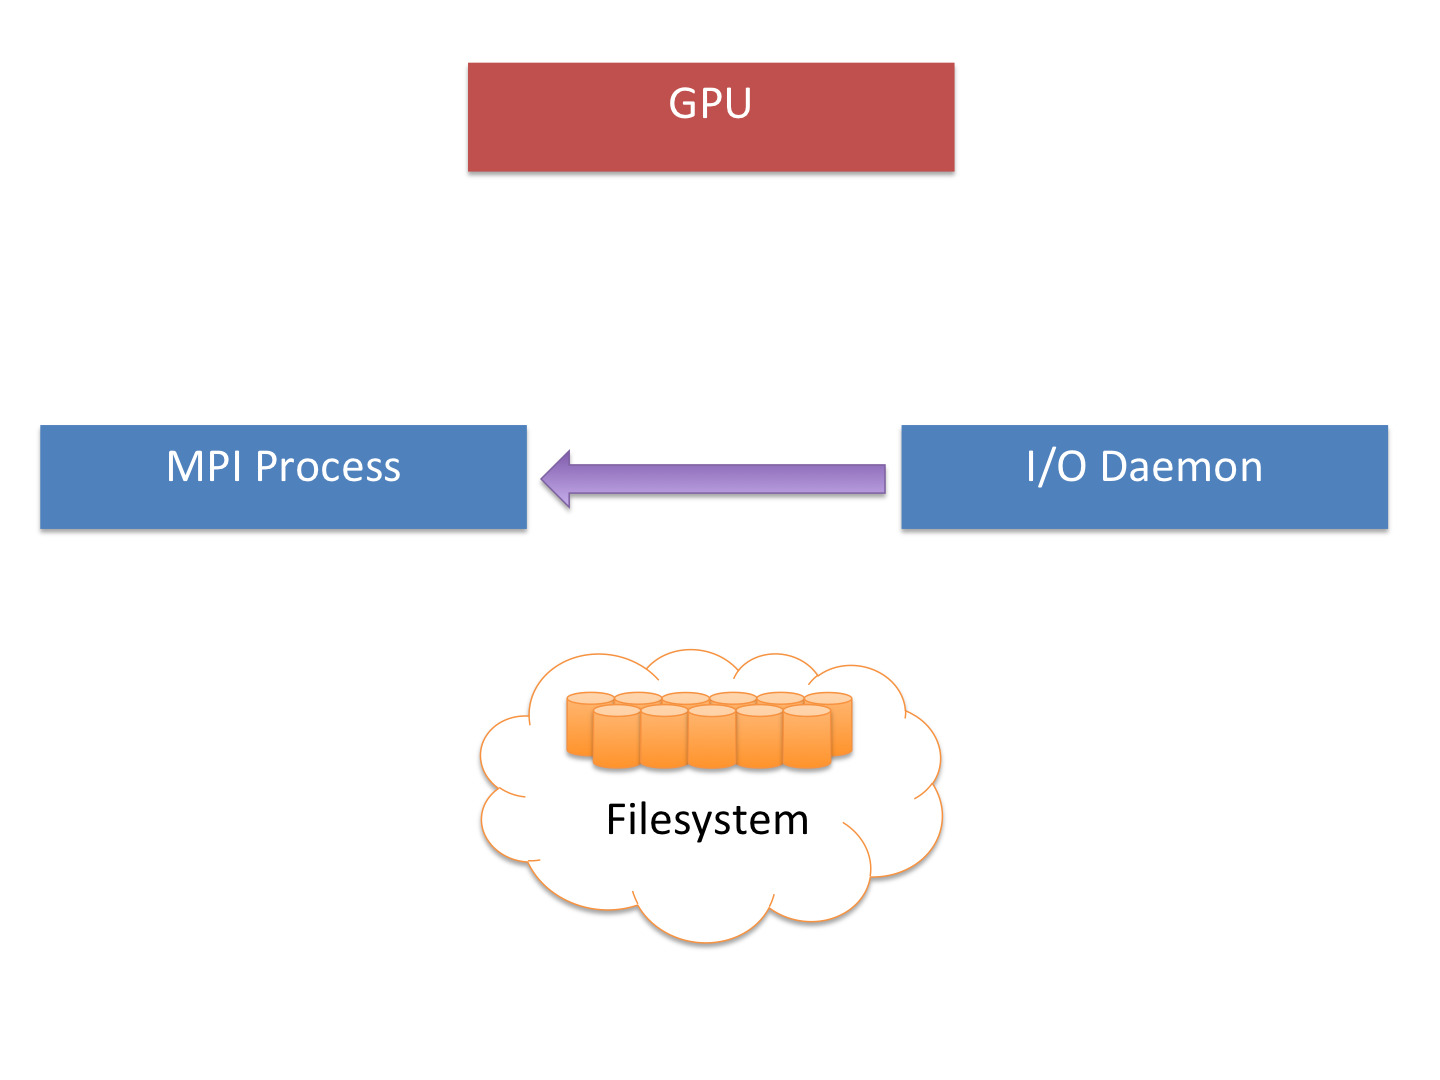
\includegraphics[width=2.5in]{figures/Data_Movement/Slide11}%
    \label{fig:comm_c}}
  \hfil
  \subfloat[Application writes data to GPU memory]{
    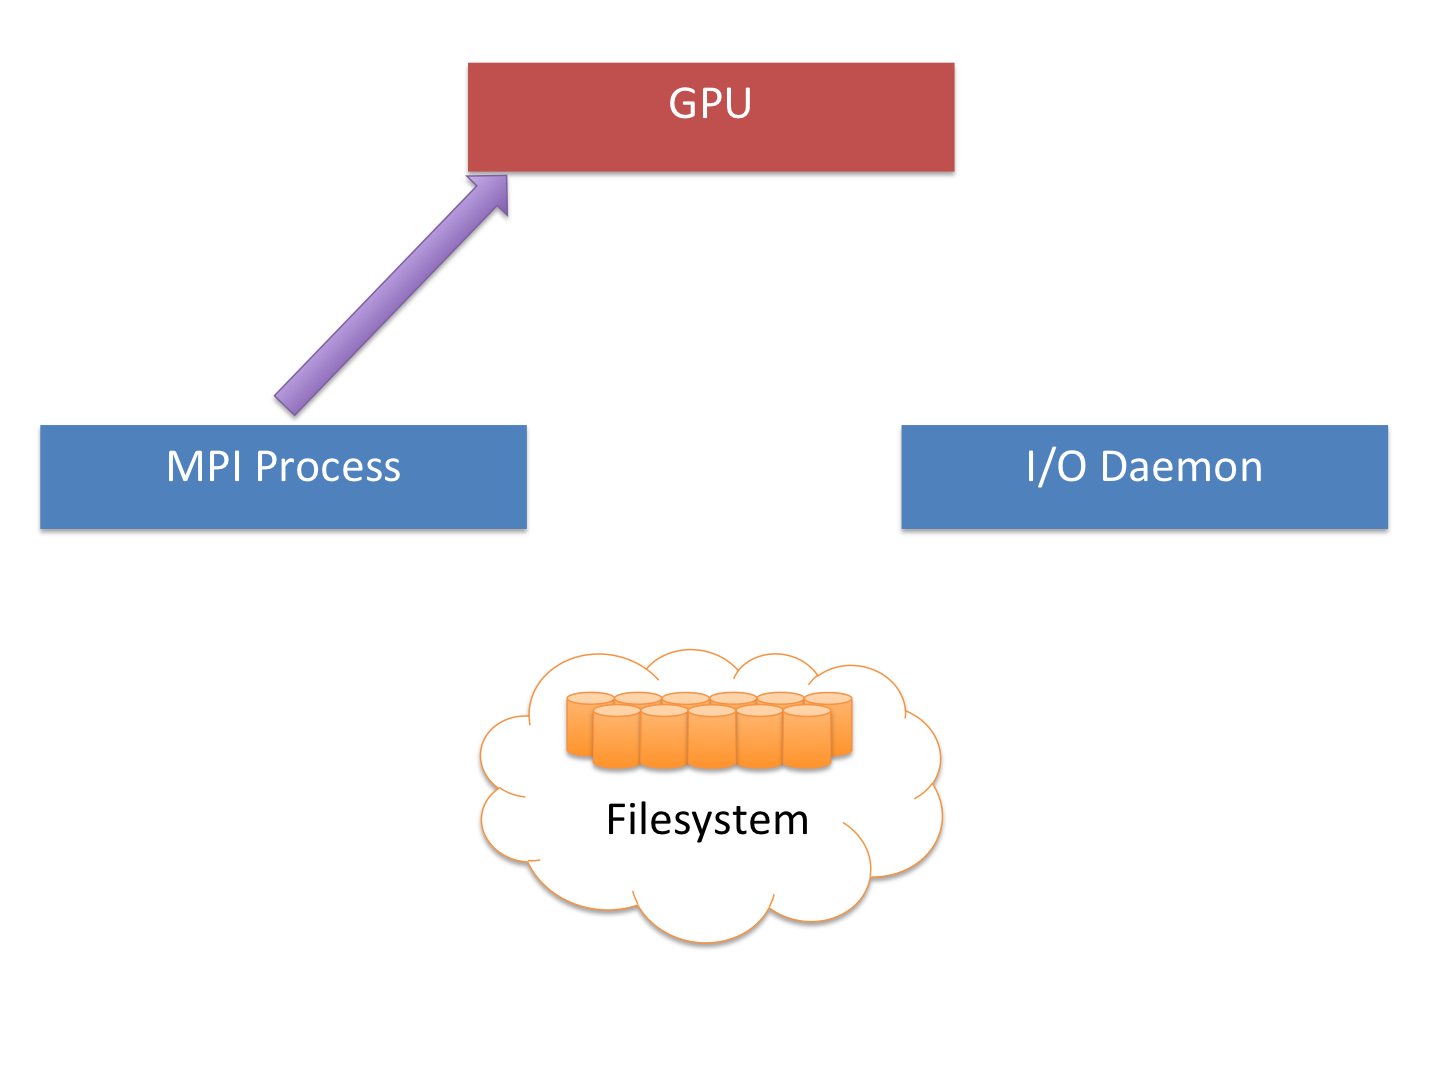
\includegraphics[width=2.5in]{figures/Data_Movement/Slide12}%
    \label{fig:comm_d}}}    
\centerline{
  \subfloat[Application sends write complete message to daemon]{
    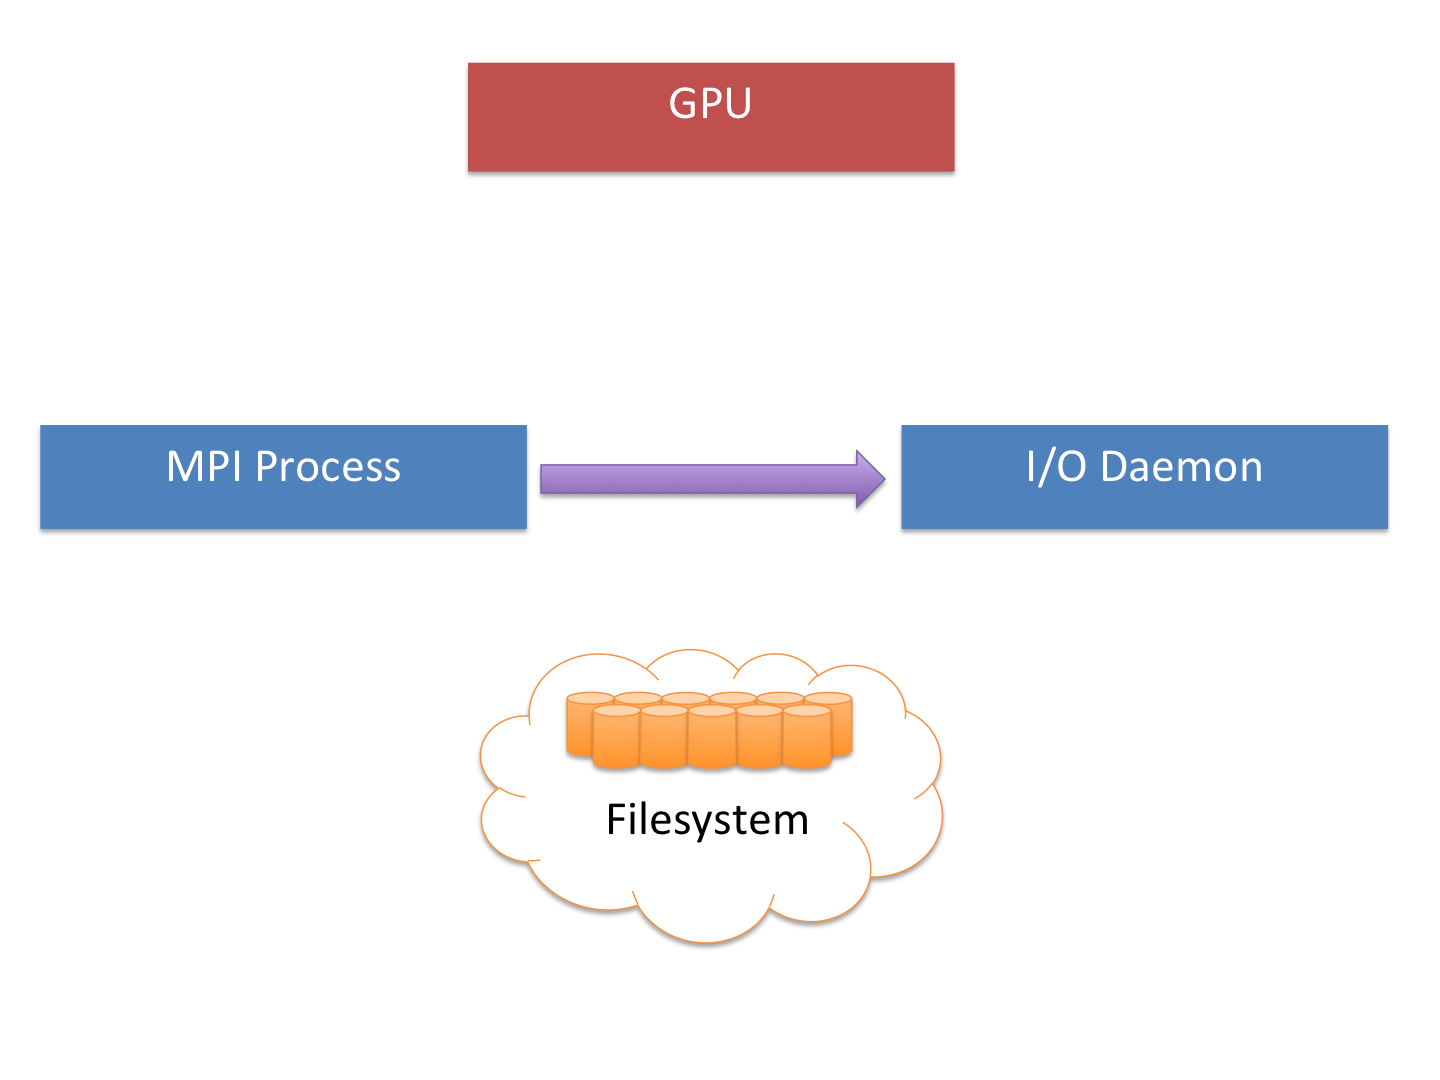
\includegraphics[width=2.5in]{figures/Data_Movement/Slide13}%
    \label{fig:comm_e}}
  \hfil
  \subfloat[Daemon copies data from GPU memory to system memory]{
    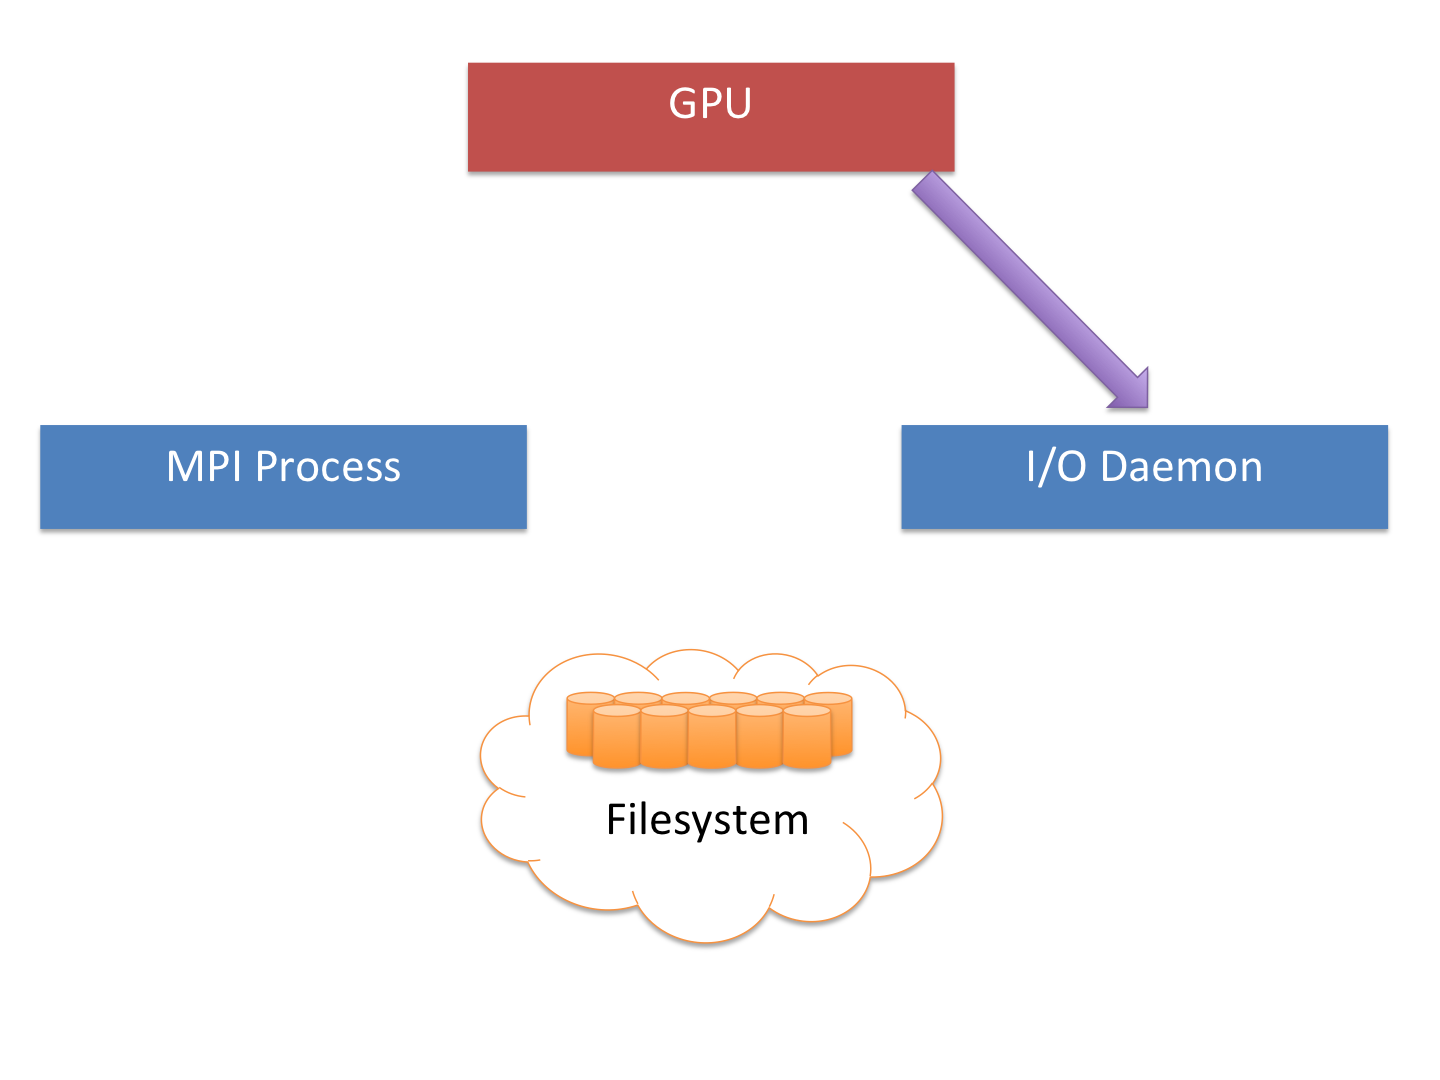
\includegraphics[width=2.5in]{figures/Data_Movement/Slide14}%
    \label{fig:comm_f}}} 
\centerline{
  \subfloat[Daemon writes data to filesystem]{
    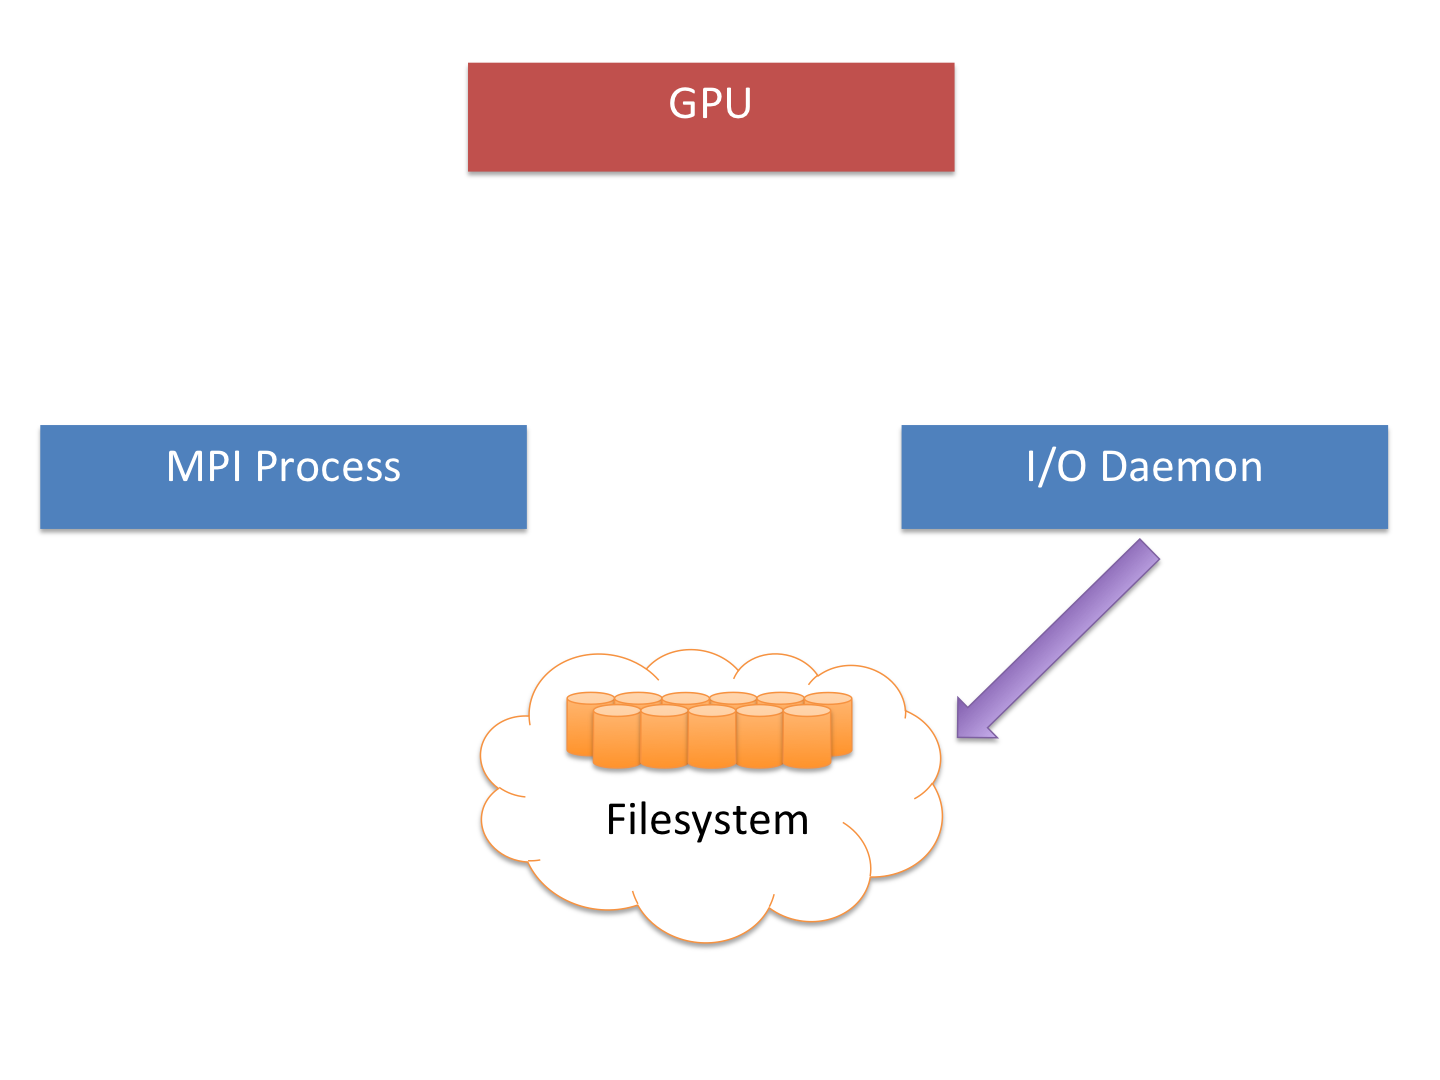
\includegraphics[width=2.5in]{figures/Data_Movement/Slide15}%
    \label{fig:comm_g}}} 
\caption{Communications steps}
\label{fig_sim}
\end{figure*}





When it's time to write, the application sends a short message to the daemon.  This message is a request to write data, and contains the amount of data and the starting offset into the output file.\footnote{For this benchmark, the daemon names output files based on the MPI rank of the requestor.  For production code, something more flexible will obviously be needed.}
\todo[inline]{We need a diagram showing the communication between the processes.}  The daemon will attempt to allocate memory on the GPU.  The daemon will then reply to the application with the size of memory that was actually allocated and a memory handle that the application can use to access the GPU memory.  Note that the size value may be less than what the application asked for.

Upon receiving the reply, the application opens the CUDA memory handle and copies the specified amount of data up to the GPU memory.  When the copy has completed, the application closes the memory handle and sends a message back to the daemon say that this particular write has completed.  If the application has more data to write, it can send another write request, or else it can continue with its calculations.

Note that the data has not made it out to the filesystem yet; it's just sitting in GPU memory.  Upon receiving the 'write done' message from the application, the daemon now knows it's free to 

The daemon maintains one or more background threads that are responsible for copying data out of GPU memory into normal system memory and then writing that data to the filesystem. 

The background write thread(s) operates asynchronously.

Each thread copies data out of GPU memory and into a buffer in system memory.  From there, it is written out to the filesystem.  The system memory buffer is deliberation kept fairly small - 16MB - in order to conserve resources.  Testing done on Titan shows that 16MB block sizes are large enough for cudaMemcpy() to give good performance.\cite{ac_guide}  Larger buffers would simply use up memory without improving performance noticeably. 


\todo[inline]{Do we need to get into the details of cuda IPC functions? cudaIpcGetMemHandle, cudaIpcOpenMemHandle, cudaIpcCloseMemHandle}


From the application's point of view, the write has completed once the 'write done' message has been successfully sent.


Once the applications sends the 'write done' message

\todo[inline]{Need to mention CCI - short messages, low latency.  Citation reference is "atchley11:cci"}

The GPU attempts to perform some load-balancing by restricting the amount of memory allocated for any single request.  Currently this limit is 16MB.  If an application wants to write 512MB, it will therefore have to make 32 separate requests.  If other ranks on the node are trying to write at the same time, their requests will all be interleaved and hopefully rank will be starved.

It's debatable whether this sort of load balancing is necessary or even desirable.  Indeed, preliminary testing seemed to indicate that it might be faster to let the daemon allocate  as much GPU memory as the client requested (assuming there was enough free).  However, that same testing showed that one of the CUDA functions - cudaIpcOpenMemHandle() - became unreliable once GPU memory allocations exceeded 512MB.  Until the nature of that problem could be determined, it was decided to limit allocations to 16MB.


\subsection{Cray-Specific Details}
\label{subsec:cray-specific}

\todo[inline]{Need an introduction paragraph for this subsection.}
The CUDA runtime can be configured to limit access to the GPU to a single thread, to multiple threads from a single process or to multiple threads from multiple processes.  On Titan, if no special options are given to qsub, the CUDA runtime will be configured for a single thread.  Since software described in this paper requires access to the GPU from multiple processes, users must switch to the appropriate compute mode.  This is done by passing the flag "-l feature=gpudefault" to qsub.\footnote{It may seem strange to have to explicitly switch to a mode called 'gpudefault'.  The naming scheme comes from the CUDA documentation.  On a standard CUDA install, the GPU would in fact default to allowing access from multiple processes.  Titan is configured differently, however.  Thus the need to explicitly tell qsub to switch to the 'default' mode.}

\todo[inline] {talk about actually starting up the daemon - fork(), open(excl), exec() }